
\section{Grundlagen}
\subsection*{Karyotyp} \index{Karyotyp} 
Ein Karyotyp ist ein Präparat des vollständigen Metaphasensatzes der Chromosomen in den Zellen einer Art oder eines einzelnen Organismus, sortiert nach Länge, Centromerlage und anderen Merkmalen.

\subsection*{Zellteilung}
\textbf{Mitose}: 2n×2 = 4n -> 2 × 2n \\
\textbf{Meiose}: 2n×2 = 4n -> × 1n

\subsection{Genome exclusion} 
% TODO
\section{Organisation des Kerngenoms von eukaryontischen Zellen}
\index{Genom!Kern}
\begin{itemize}
    \item Im Kern
    \item Kerngenome bestehen aus Chromosomen, die ein lineares DNA Molekül beinhalten 
\end{itemize}
\subsection{Nukleosomen} \index{Nukleosom}
\begin{mechanism}[title=Definition Nukleosom]
Grundlegende Strukturelle Einheit der Eucaryotischen Chromosomen. Sie bestehen aus einem Komplex aus DNA und Histonen.
\end{mechanism}
\begin{multicols}{2}
\begin{figure}[H]
    \centering
    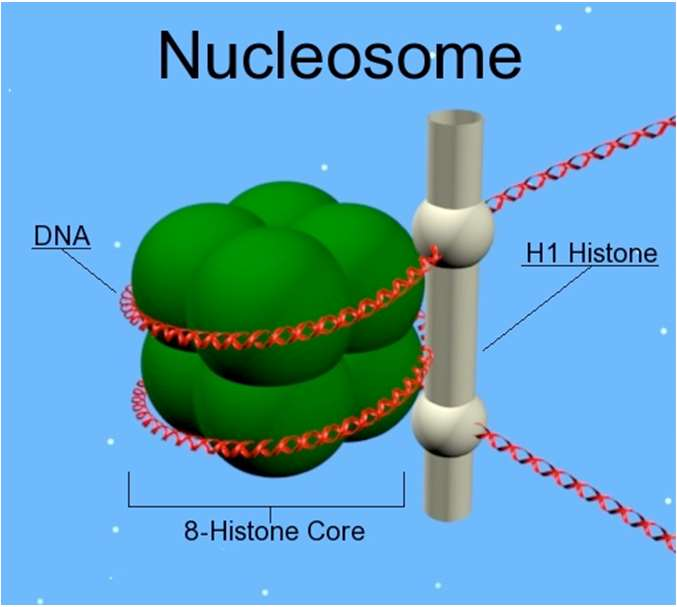
\includegraphics[width=8cm]{images/chomatosom.jpg}
    \caption{Chromatosom.}
    \label{fig:chomatosom}
\end{figure} \index{Chromatosom}

\columnbreak
\noindent Komplex aus DNA und Histonen, erste Verpackungsstufe der DNA im Zellkern eukaryotischer Zellen. \\ \index{Histon} \index{Verpackungsstufen}
Besteht aus: 
\begin{itemize}
    \item DNA
    \item 2 × H2A
    \item 2 × H2B
    \item 2 × H3
    \item 2 × H4 
\end{itemize}
Zusammen mit dem Linker Histon H1 bezeichnet man das Nukleosomen Core Partikel inklusive Linker DNA als Chromatosom. \index{Nukleosom} \index{Chromatosom} \index{Histon} \index{Histon!H1}
\end{multicols}
\subsubsection{Dynamische Bindung von H1 an Chromatin}
\begin{enumerate}
    \item \textbf{Schritt}: H1 "kommt an"
    \item \textbf{Schritt}: Bindet unspezifisch an Linker DNA
    \item \textbf{Schritt}: Runde Domöne des H1 positioniert sich auf/an dem Nukleosom
    \item \textbf{Schritt}: Strukturelle Veränderungen des Chromatins
\end{enumerate}
HMG = high mobility group.


\section{Epigenetik}
\begin{mechanism}[title=Definition Epigenetik]
Epigenetik ist die Lehre von den \textbf{vererbbaren Veränderungen} des Phänotyps, die \textbf{nicht mit Veränderungen der DNA-Sequenz einhergehen}. 
\end{mechanism} \index{Epigenetik}
\noindent Epigenetik bezieht sich auf \textbf{stabile Veränderungen} in der Regulierung der Genexpression, die während der Entwicklung, Zelldifferenzierung und Zellproliferation auftreten und über Zellteilungen hinweg etabliert und aufrechterhalten werden, ohne dass die DNA-Sequenz verändert wird.
% Waddington‘s Epigenetic Landscape rausgelassen (F14) & The epigenetic pinball machine /(F15)
Epigenetische Mechanismen: 
\begin{itemize}
    \item Kovalente Modifikation
    \item RNA-Transkripte
    \item Micro-RNAs
    \item mRNA \index{RNA!mRNA}
    \item sRNA \index{RNA!sRNA}
    \item Prione \index{Prion}
    \item Histon-Varianten
\end{itemize}

\subsection{DNA-Methylierung} \index{Methylierung} \index{DNA!Methylierung}
Takeaway: Nur Cytosin und Adenin, können methyliert werden! \\
Cytosin-Methylierung ist in Eukaryoten und Prokaryoten weit verbreitet und der Grad der Methylierung kann sich zwischen Spezies stark unterscheiden. \\ \index{Methylierung!Cytosin}
Funktionsweise: Übertragung von Methylgruppen durch Enzyme (DNA-Methyltransferasen) auf Nukleobasen \\
Methylierungsmuster werden während der Replikation durch die Erhaltungs-DNMT1 bewahrt \\ \newline \index{DNMT1} \index{Methylierungsmuster} \index{Methyltransferasen}
Bei Säugetieren ist die DNA-Methylierung für eine normale Entwicklung unerlässlich und wird mit einer Reihe von Schlüsselprozessen in Verbindung gebracht einschließlich genomischer Prägung, Inaktivierung des X-Chromosoms, Unterdrückung von transponierbaren Elementen, Alterung und Karzinogenese.
\begin{mybox}[title=Passive und aktive Demythilierung]
Passive Demethylierung erfolgt während der DNA-Replikation und ist ein Prozess, bei dem Methylgruppen auf der DNA nicht aktiv entfernt werden, sondern durch die DNA-Replikation verloren gehen. \\
Aktive Demethylierung ist ein biochemischer Prozess, bei dem Methylgruppen aktiv von der DNA entfernt werden. Dieser Prozess erfordert Enzyme und ist nicht von der DNA-Replikation abhängig. \index{Demythilierung} \index{Methylierung}
\end{mybox}
\begin{table}[H]
    \begin{tabular}{p{8cm}p{8cm}}
        \textbf{Normale Zellen} & \textbf{Krebszellen}  \\ \\
        CpG-Inseln sind resistent gegen DNA-Methylierung & CpG-Inseln sind anfällig für DNA-Hypermethylierung \\ \\
        -> usgewogenes Methylierungsmuster reguliert Genexpression & -> abnormes Gen-Silencing, genomische Instabilität, abnormale Gen-Expression 
    \end{tabular}
    \caption{Vergleich von DNA-Methylierungsmuster in normalen und Krebszellen}
    \label{tab:methylierungkrebs}
\end{table} \index{CpG-Inseln} \index{Methylierungsmuster}
\subsection{Histonmodifikation} \index{Histonmodifikation}
\begin{mechanism}[title=Beispiele von epigenetischen Modifikationen an Histonen]
\begin{itemize}
    \item Acetylierung
    \item Methylierung
    \item Ubiquitinierung von Lysin
    \item Phosphorylierung von Serin- und Threoninresten
\end{itemize} \index{Histonmodifikation} \index{Phosphorylierung} \index{Ubiquitinierung} \index{Acetylierung} \index{Methylierung}
\end{mechanism}

In Krebszellen sind die Muster der Histonmodifikationen oft gestört. Es kann eine globale Hypoacetylierung oder Hypermethylierung bestimmter Gene auftreten, insbesondere von Tumorsuppressorgenen. \index{Acetylierung!Hypo} \index{Methylierung!Hyper}
\begin{table}[H]
    \begin{tabular}{p{4cm}p{6cm}p{6cm}}
        & \textbf{Heterochromatin} & \textbf{Euchromatin}  \\
        Methylationslevel & Hoch  &  Variable \\
        Methylierungsumsatz & Niedrig  & Hoch 
    \end{tabular}
    \caption{DNA-Methylierungsumsatz in Heterochromatin und Euchromatin.}
    \label{tab:methylheteroeu}
\end{table} \index{Heterochromatin} \index{Euchromatin}

\section{Genomorganisation bei Eukaryoten}
\begin{mechanism}[title=Kodierendes Eukaryonten Gen beschriften]
\begin{figure}[H]
    \centering
    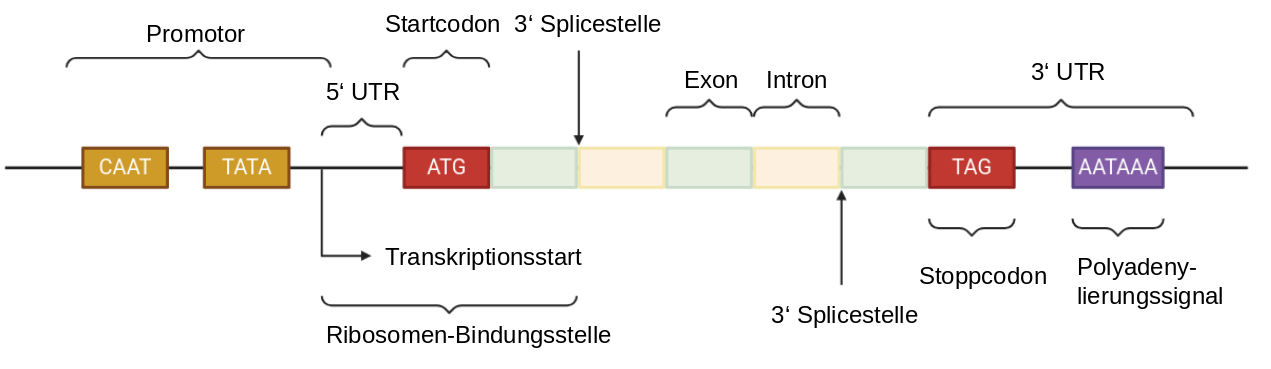
\includegraphics[width=12cm]{images/eukgenfilled.png}
\end{figure}
\end{mechanism}
Es gibt verschiedene Modelle der Chromatinorganisation! %Folie  24
\begin{figure}[H]
    \centering
    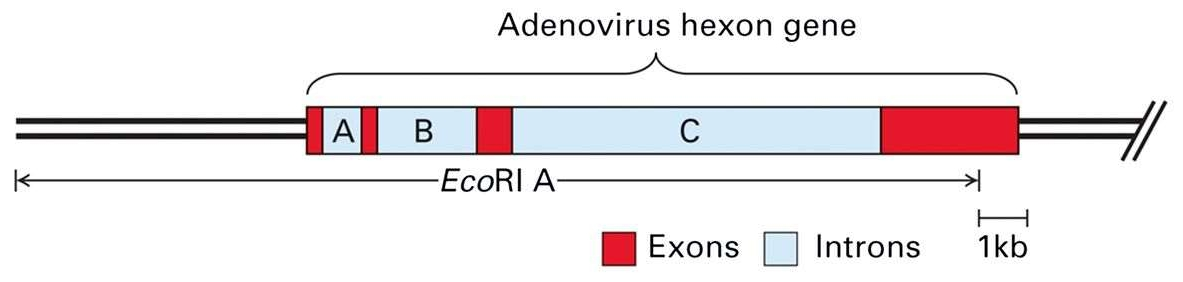
\includegraphics[width=8cm]{images/mosaikstruktur.jpg}
    \caption{Moasikstruktur.}
    \label{fig:mosaikstruktur}
\end{figure} \index{Moasikstruktur}
\noindent Takeaway: Eukaryotische Gene haben Introns und die unterbrechen die codierenden Regionen \index{Intron}
\subsubsection{Genomgrößen}
Takeaway: Die Größe eukaryontischer Genome und die evolutionäre Entwicklung korrelieren NICHT miteinander! \\
Eukaryotische Genomgrößen und geschätzte Genzahlen korrelieren NICHT (\gls{C-Wert}-Paradoxon)! \\ \index{C-Wert-Paradoxon} % Protein coding capacity 
\noindent Eukaryotische Genome enthalten einen geringen Anteil an Regionen, die für Proteine kodieren! -> Rest sind repetetitive ("Müll"-)Sequenzen 
% Teils Rausgelassen was diese Repeats sein könenen (F34)
U.a.: 
\begin{itemize}
    \item \glspl{Transposon} \index{Transposon}
    \item Simple sequence repeats/microsatellites \index{Microsatellit}
    \item ...
\end{itemize}
\begin{mechanism}[title=Definition Transposon]
Mobile genetische Elemente und können sich von einem Ort im Genom zu einem anderen bewegen, entweder durch einen "Kopieren-und-Einfügen"-Mechanismus oder durch einen "Ausschneiden-und-Einfügen"-Mechanismus.
\end{mechanism}
\subsubsection{Unter-Genome}
\begin{mechanism}[title=Bennen Sie die drei (Sub)Genome einer eukaryotischen Zelle]
\begin{itemize}
    \item Nukleom: Kern-Genom \index{Nukleom}
    \item Chondriom: Mitochondrium-Genom (variabel in Größe und Struktur) \index{Chondriom}
    \item Plastom: Chloroplasten-Genom (gleichbleibende allgemeine Struktur) \index{Plastom}
\end{itemize}
\end{mechanism}
\begin{mechanism}[title=Welches Genom gibt es nur in Pflanzenzellen?]
Plastom
\end{mechanism}
\begin{mechanism}[title=Was weißt auf den prokaryotischen Ursprung einiger dieser Genome hin?]
Organellengenome weisen Merkmale auf, die an prokaryotische Genome erinnern (Endosymbiontentheorie). \\
Genomische Analysen zeigen, dass viele Gene in Mitochondrien und Chloroplasten eine enge Verwandtschaft mit Genen von bestimmten Gruppen von Bakterien aufweisen, wie Alphaproteobakterien im Fall von Mitochondrien und Cyanobakterien im Fall von Chloroplasten.
\end{mechanism}

\subsection{Retrotransposonen} \index{Retrotransposonen}
Retroviren sind behüllte Viren. Anders als bei „normalen“ RNA-Viren aber muss die RNA von Retroviren zunächst einmal mittels reverser Transkription in ein DNA-Molekül umgeschrieben werden, bevor sie als solches in das Genom der Wirtszelle eingebaut und dort aktiv werden kann. 
\subsubsection{\gls{line}} \index{LINE} \index{Retrotransposon!Nicht-LTR}
Gruppe von Nicht-LTR-Retrotransposonen, weit verbreitet im Genom vieler Eukaryoten - hat zwei seperate \glspl{orf} und ca. 6000bp. 
\subsubsection{\gls{sine}} \index{SINE}
Revers-transkribierte RNA-Moleküle, die ursprünglich von der RNA-Polymerase III in tRNA, 5S ribosomale RNA und andere kleine Kern-RNAs umgeschrieben wurden. Kodieren nicht für ein funktionsfähiges Reverse-Transkriptase-Protein und sind <500 bp.
\subsubsection{Alu-Element} \index{Alu-Element}
Sind die häufigsten SINEs bei Primaten. \index{SINE}



\section{Replikation}
Takeaway: Das letzte Okazaki-Fragment kann während der DNA-Replikation nicht geprimed werden -> \gls{Lagging Strand Copy} -> Geninformationen gehen verloren.  \index{Okazaki-Fragment} \index{Lagging Strand Copy}
\begin{mybox}[title=Wieso kann das letzte Okazaki-Fragment nicht geprimed werden?]
Um mit der Synthese eines Okazaki-Fragments zu beginnen, benötigt die DNA-Polymerase einen Primer, der von der Primase synthetisiert wird. edes Okazaki-Fragment wird also durch einen neuen RNA-Primer initiiert, der in der Nähe des vorherigen Okazaki-Fragments platziert wird. Wenn sich die Replikationsgabel dem Ende des DNA-Strangs nähert, bleibt möglicherweise nicht genügend Platz oder keine geeignete Vorlage für die Primase, um einen Primer für das letzte Okazaki-Fragment zu setzen.\\ In Eukaryoten wird das Problem in der Regel durch spezielle Enzyme gelöst, die die Lücken füllen, nachdem die RNA-Primer entfernt wurden.
\end{mybox}
\begin{figure}[H]
    \centering
    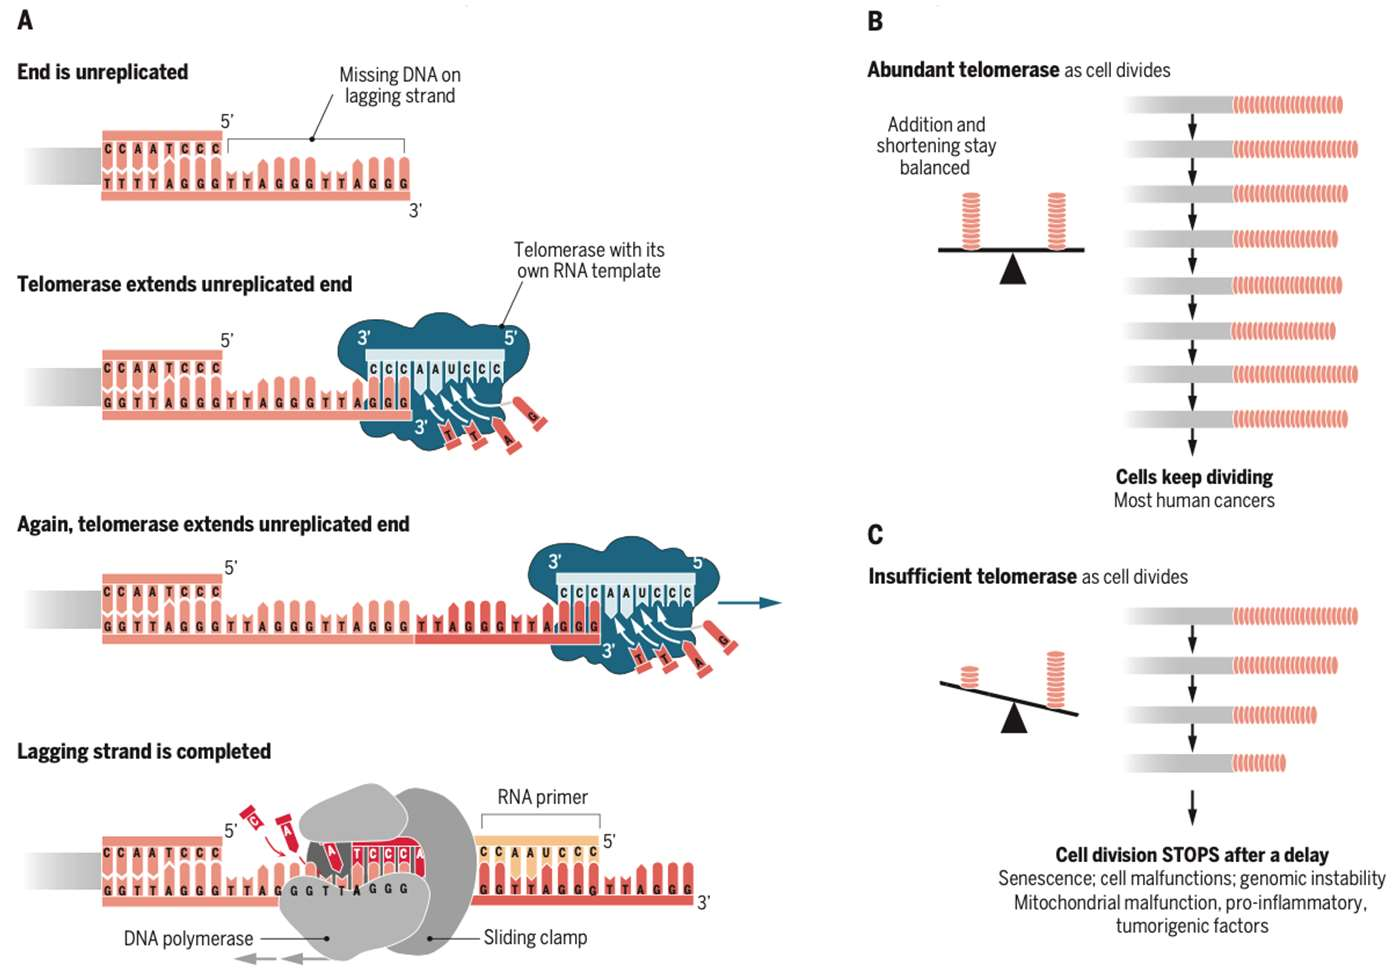
\includegraphics[width=8cm]{images/telomerase.jpg}
    \caption{Funktionsweise der Telomerase.}
    \label{fig:telomerase}
\end{figure} \index{Telomerase}
\noindent Takeaway: Die langfristige Aufrechterhaltung der telomeren DNA-Länge erfordert \gls{telomerase}! \\
\gls{telomerase} erkennt das 3'-OH am Ende des \gls{G-Strang-Überhang}s \\
TRF = telomere repeat binding factor 
\section{Model-Pflanzen und ihre Relevanz}
Guter Model-Organismus: \index{Model-Organismus}
\begin{itemize}
    \item kleines Genom 
    \item wenige repetitive Sequenzen im Genom 
    \item Einfache Haltung
    \item Kurze Generationszeit 
    \item nahe verwandt mit relevanten Organismen 
    \item Verfügbarkeit von Werkzeugen für genetische Manipulationen
\end{itemize}
\section{Kartierung} \index{Kartierung}
\subsection{\gls{rflp}}
Um genetische Variationen zwischen Individuen zu analysieren und zu kartieren. \\
Die isolierte DNA wird mit Restriktionsenzymen behandelt. Die Längen der DNA-Fragmente, die bei verschiedenen Individuen oder Proben entstehen, werden verglichen. Unterschiede in der Fragmentlänge deuten auf Variationen in der DNA-Sequenz hin. \index{Restriktionsenzym}
\subsection{Southern hybridization / Southern Blot} \index{Southern Blot}
Kann mophologische und molekulare Marker kartieren. \\
Ermöglicht den Nachweis einer Gensequenz in einem komplexen DNA-Gemisch (z. B. dem gesamten Genom eines Organismus) innerhalb kurzer Zeit, ohne dass sämtliche Sequenzen des Gemisches entschlüsselt werden müssen.
\begin{figure}[H]
    \centering
    \begin{subfigure}[t]{12cm}
        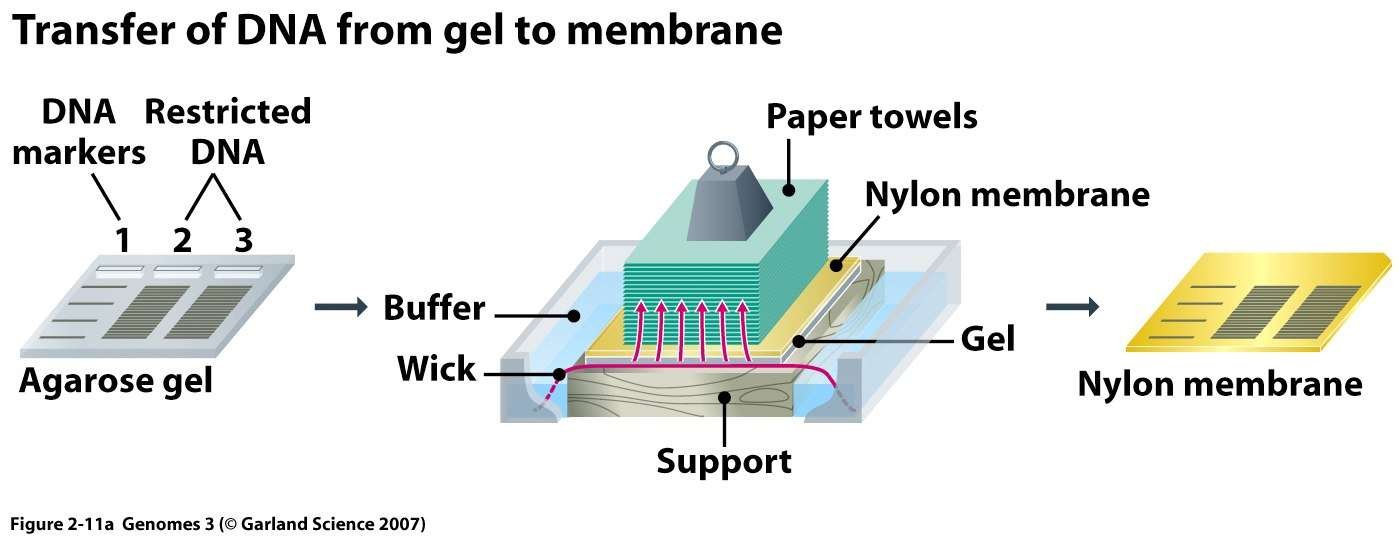
\includegraphics[width=\textwidth]{images/souther1.jpg}
        \caption{Caption}
        \label{fig:souther1}
    \end{subfigure}
    \begin{subfigure}[t]{12cm}
        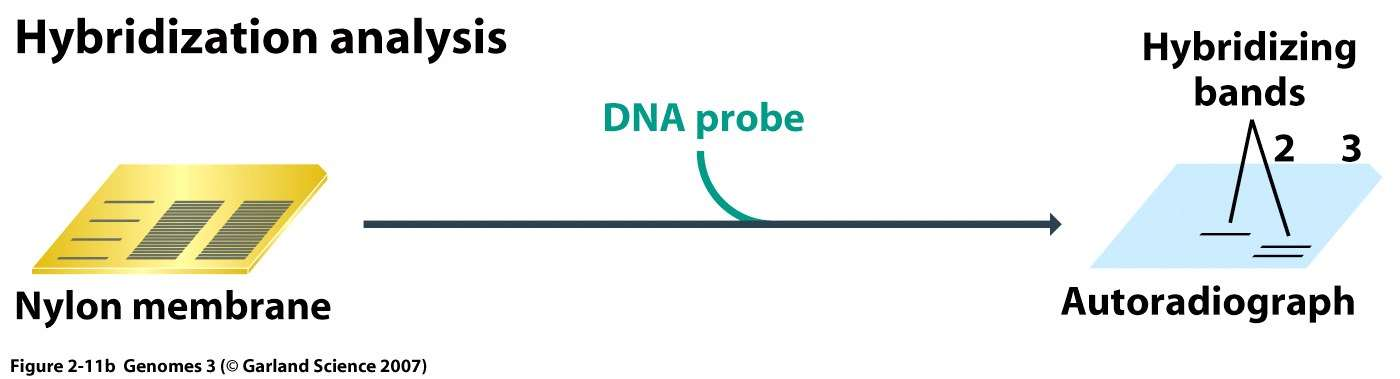
\includegraphics[width=\textwidth]{images/souther2.jpg}
        \caption{Caption}
        \label{fig:souther2}
    \end{subfigure}
    \caption{Caption}
    \label{fig:southernblot}
\end{figure}
\begin{mechanism}[title=Was ist Southern Blot? Erkläre das Prinzip.]
Schneller Nachweis einer Gensequenz in einem Genom durch das Übertragen der durch Gelelektrophorese aufgetrennten DNA-Fragmente auf eine Membran und anschließender Hybridisierung der Ziel-Sequenzen mit markierten Sonden. 
\end{mechanism}
\begin{mechanism}[title=Erklären Sie die wichtigsten Bestandteile von Souther Hybridisierung]
\begin{enumerate}
    \item DNA-Extraktion und -Aufbereitung (Reinigung)
    \item Restriktionsenzym-Verdau
    \item Gelelektrophorese
    \item Denaturierung
    \item Transfer auf eine Membran
    \item Hybridisierung mit einer markierten Sonde
    \item Waschen
    \item Detektieren
\end{enumerate}
Bestandteile: Papiertücher, Nylonmenbran, Gel Puffer, Support, Schnur, Kammer

\end{mechanism}
\subsection{Ökotypen (Ecotypes)} \index{Ökotyp}
Untergruppen (Sippen) einer Art, die im Vergleich zu anderen Populationen der gleichen Art eigene genetisch fixierte ökologische Ansprüche an ihre Umwelt stellen. Die Ökotypen sind häufig auf ein Teilareal einer Art beschränkt und kommen nur bei bestimmten Umweltbedingungen vor. \\
Weisen phänotypische und genetische Polymorphismen auf und diese Polymorphismen bilden die Grundlage für die genetische Kartierung.


\subsection{SNP-Typisierung durch Oligonukleotid-Hybridisierungsanalyse} \index{SNP-Typisierung} \index{Oligonukleotid-Hybridisierungsanalyse}
\subsubsection{\gls{sslp}}
\glspl{sslp} sind Arrays von repetitiven Sequenzen, die Längenvariationen aufweisen, wobei die verschiedenen Allele eine unterschiedliche Anzahl von Wiederholungseinheiten enthalten.
\begin{itemize}
    \item \textbf{Minisatelliten}: \glspl{vntr} - bis 25bp \index{Minisatellit}
    \item \textbf{Microsatelliten}: \glspl{str} - 13bp oder weniger \index{Microsatellit}
\end{itemize}
\subsubsection{\glspl{snp}}
 Geerbte und vererbbare Variation eines einzelnen Basenpaares in einem komplementären DNA-Doppelstrang.
\subsubsection{Oligonukleotid-Hybridisierungsanalyse} \index{Oligonukleotid-Hybridisierungsanalyse}
Prinzip: Wenn alle Basen zweier DNA-Stränge sind paaren können (sie komplmentär sind), ist das stabil und wenn sich in einem Strang (min) eine Base unterscheidet, ist es nicht stabil -> erfolgreiche Hybridisierung nur bei kompletter Übereinstimmung. \\
Das überprüft man, indem man an das eine Ende Floreszenz packt und an das anderen etwas zur Fluoreszenzlöschung. \index{Fluoreszenzlöschung}
\begin{figure}[H]
    \centering
    \begin{subfigure}[t]{0.4\textwidth}
    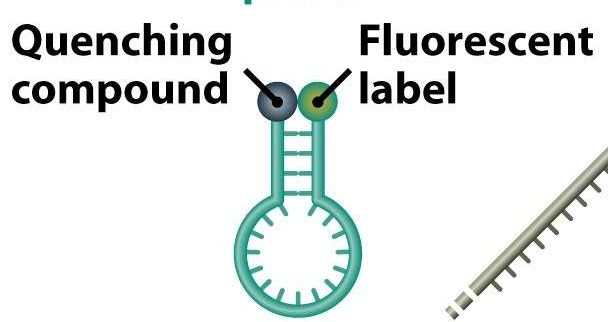
\includegraphics[width=\textwidth]{images/unhypridizedsnp.jpg}
    \caption{Wenn es nicht hypridisiert ist, bleibt es in einer Struktur, in der die Fluoreszenz durch den Fluoreszenzlöscher gelöscht wird und nicht leuchtet.}
    \label{fig:unhypridizedsnp}
\end{subfigure}
\hfill
\begin{subfigure}[t]{0.4\textwidth}
    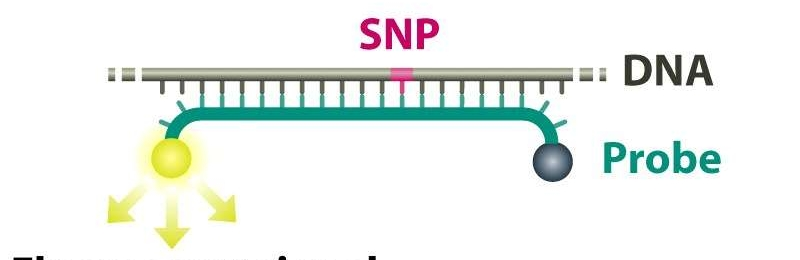
\includegraphics[width=\textwidth]{images/hybidizedsnp.jpg}
    \caption{Wenn es erfolgreich hybridisiert, werden Fluoreszenzpartikel und Fluoreszenzlöscher getrennt und es leuchtet.}
    \label{fig:hybidizedsnp}
    \end{subfigure}
    \caption{Wenn man nun die Probe mit Fluoreszenz markiert, kann man hinterher sehen, ob erfolgreich hybridisiert wurde. Weil leuchtet dann...}
    \label{fig:OligonukleotidHybridisierungsanalyse}
\end{figure} \index{Fluoreszenzlöschung} \index{Fluoreszenzpartikel} \index{Oligonukleotid-Hybridisierungsanalyse}
\begin{figure}[H]
    \centering
    \begin{subfigure}[t]{0.3\textwidth}
    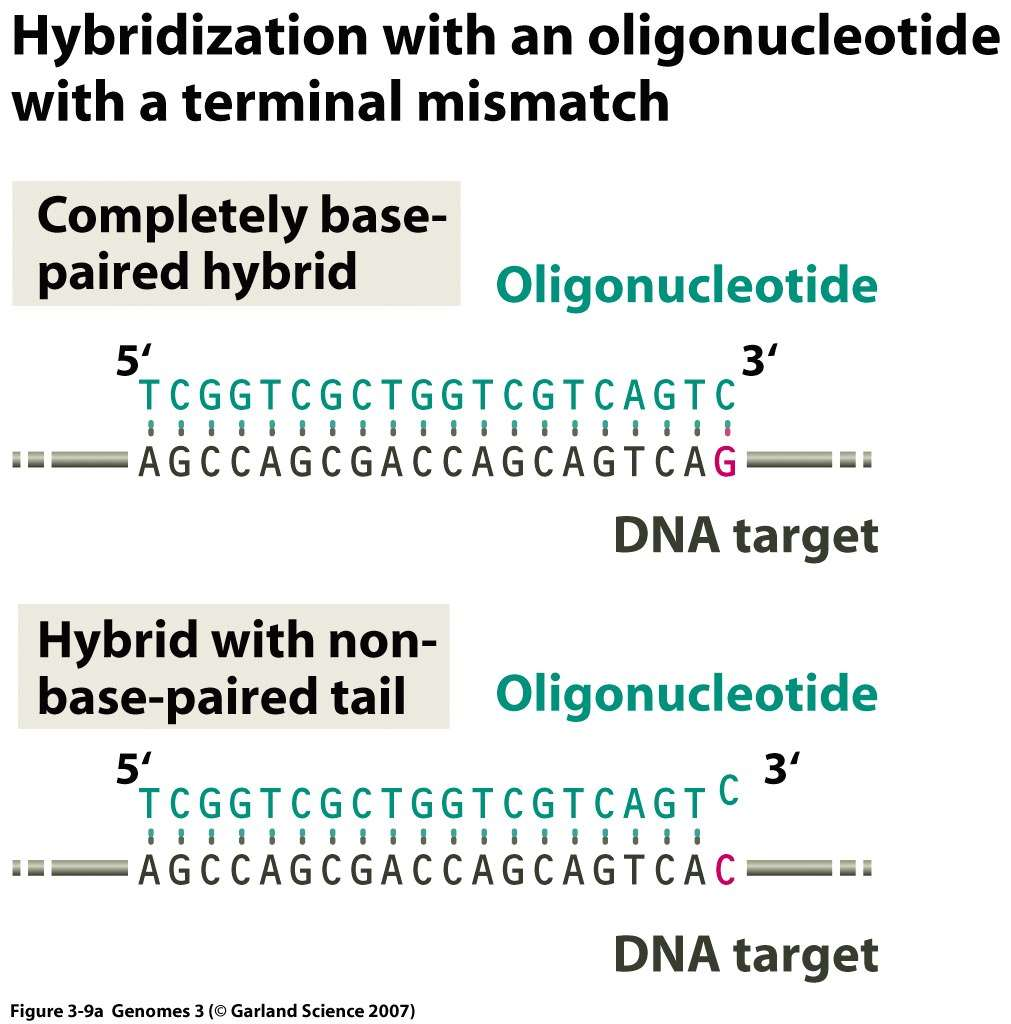
\includegraphics[width=\textwidth,height=6cm]{images/terminalmismatch.jpg}
    \caption{Terminal Mismatch-Methode: Es wird ein Oligonukleotid verwendet, das spezifisch an eine Ziel-DNA-Sequenz bindet. Wenn es ein Mismatch (eine nicht komplementäre Base) am Ende des Oligonukleotids gibt, wird die Bindung des Oligonukleotids an die Ziel-DNA beeinträchtigt. Das beenfluddt die Effizienz der Amplifikation während der PCR oder anderen nachfolgenden Schritten, was zur Detektion des SNPs führt.}
    \label{fig:terminalmismatch}
\end{subfigure}
\hfill
\begin{subfigure}[t]{0.3\textwidth}
    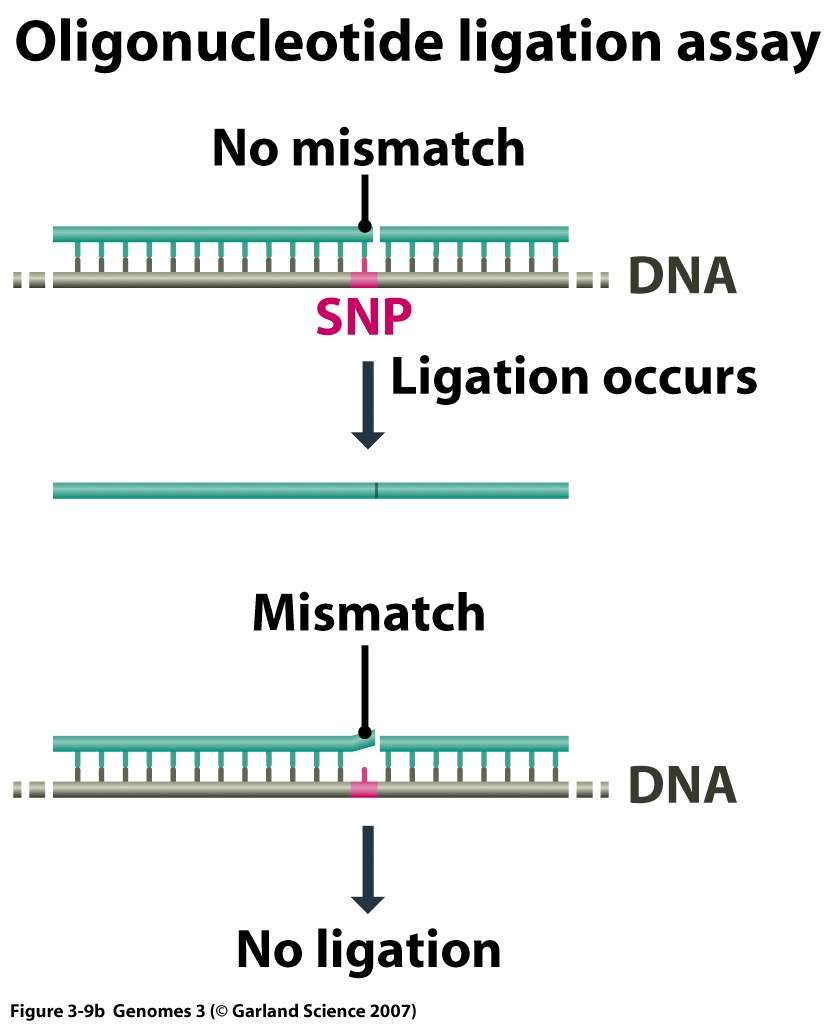
\includegraphics[width=\textwidth,height=6cm]{images/litigationassay.jpg}
    \caption{Oligonucleotide Ligation Assays (OLA): Die Oligonukleotide binden an die Ziel-DNA, die den SNP enthält. Wenn die Oligonukleotide korrekt an die Zielsequenz binden und der SNP an einer spezifischen Position liegt, können die Oligonukleotide miteinander verknüpft (ligiert) werden.}
    \label{fig:litigationassay}
    \end{subfigure}
    \hfill
    \begin{subfigure}[t]{0.3\textwidth}
    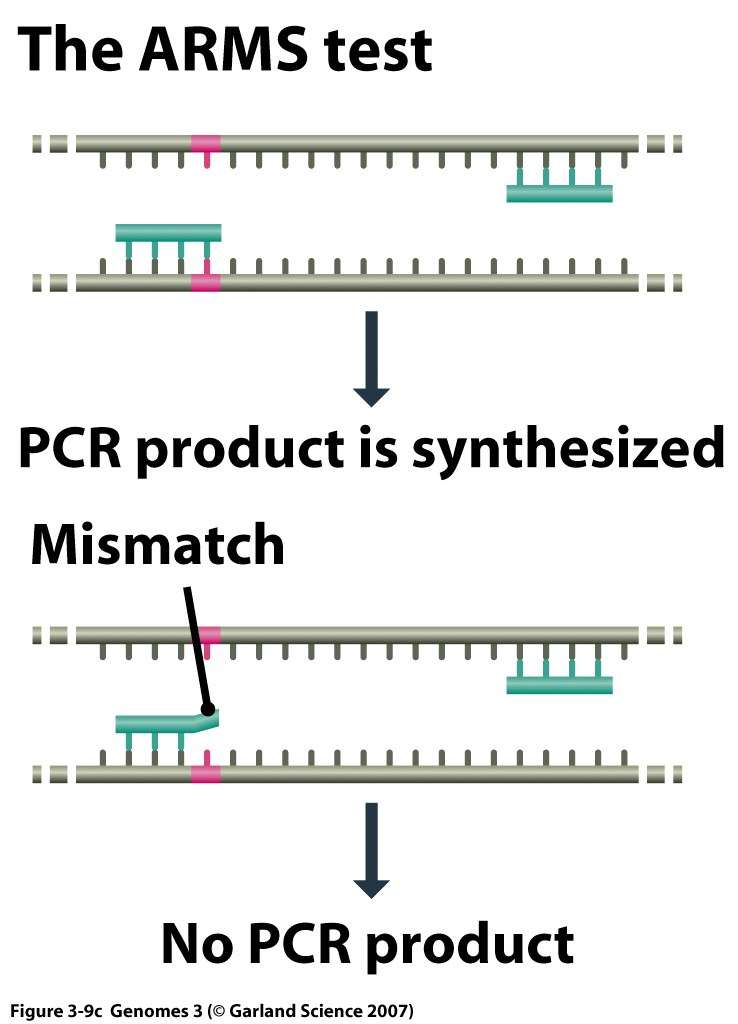
\includegraphics[width=\textwidth,height=6cm]{images/armstest.jpg}
    \caption{Amplification Refractory Mutation System (ARMS) Test: PCR-basierte Methode, die spezifische Primer verwendet, um zwischen zwei Allelen eines SNP zu unterscheiden. Es werden zwei verschiedene Primerpaare verwendet: eines für das Wildtyp-Allel und eines für das Mutations-Allel. Die Primer sind so gestaltet, dass sie nur an die Ziel-DNA binden, wenn die spezifische SNP-Variation vorhanden ist.}
    \label{fig:armstest} 
    \end{subfigure}
    \caption{Methoden der Oligonukleotid-Hybridisierungsanalyse.}
    \label{fig:OligonukleotidHybridisierungsanalyseMethoden}
\end{figure} \index{Oligonukleotid-Hybridisierungsanalyse}

\subsection{Zytogenetische Kartierung mittels FISH} \index{Kartierung!Zytogenetische}
FISH = Fluoreszenz-in-situ-Hybridisierung \\
Wird zur Pränataldiagnostik verwendet \\
"Diese Art von molekularem Test basiert auf der Verwendung von fluoreszierenden, sequenzspezifischen Sonden, die an Chromosomen hybridisieren. Diese chromosomale DNA muss hierzu in der Interphase oder der Metaphase vorliegen. Die Visualisierung erfolgt unter einem Fluoreszenzmikroskop. \\

Hiermit kann die Position der einzelnen Sequenzen der Sonden mittels Fluoreszenzmarkierung bestimmt werden, was einen Vorteil im Gegensatz zum herkömmlichen Karyogramm darstellt. Hiermit können Deletionen sowie Insertionen erkannt werden. "
